\chapter{Related work}
\fxnote{Make a list of terms}
This is not the first project attempting to visualising large raster datasets in an interactive way. 

\section{Tilebased raster visualisation}
In \citet{Baumrocks} master thesis, he created a webmap, where raster tiles were being colored locally. 

\begin{figure} [H]
	\centering
	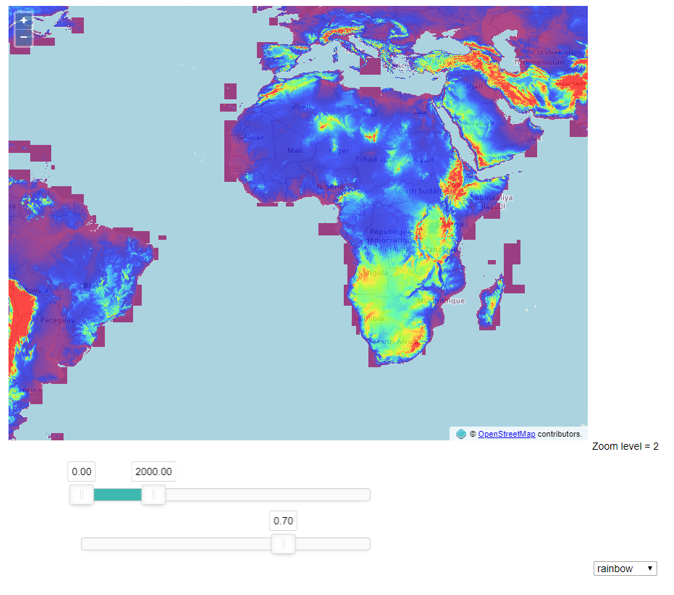
\includegraphics[width=.6\textwidth]{Pictures/BaumrockMap1}
	\caption{An elevation map, where the user can control how the raster is colored using the controls below the map. Created by \citep{EOX}}
	\label{BaumrockMap1}
\end{figure}

A picture of one of his maps can be seen in figure \ref{BaumrockMap1}. This particular map is not included in his thesis, but it is the most similar to this project. The map shows an elevation data . Below the map are two sliders and a dropdown list with the label “viridis”. Changing the value in this dropdown list allows the user to switch to another color scheme. The bottom slider is controlling the opacity for the raster layer. The upper slider controls which maximum and minimum values the coloring should be based on. How the map change, when changing the values in the upper slider can be seen in figure \ref{BaumrockMap2}. When zooming in another more detailed layer gets loaded and rendered.
\begin{figure} [H]
	\centering
	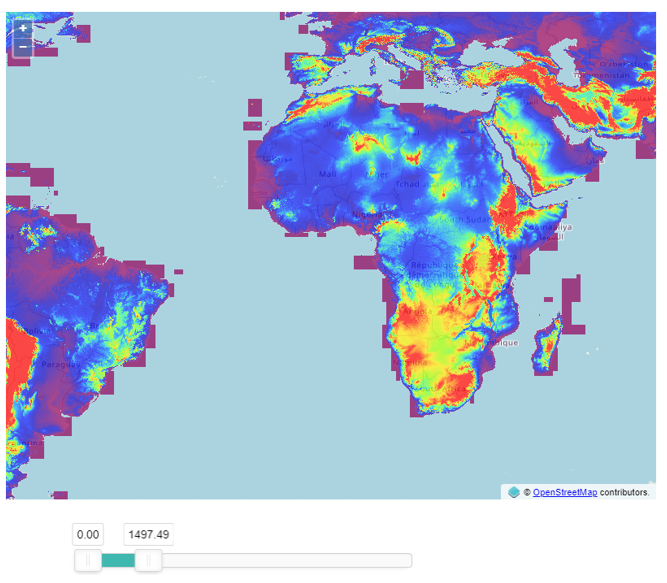
\includegraphics[width=.6\textwidth]{Pictures/BaumrockMap2}
	\caption{How the map change, when using the slider}
	\label{BaumrockMap2}
\end{figure}

When taking a closer look at the source code it can be seen that the raster is being loaded as tiff tiles with a bit depth of 16 bit. \citep{EOX} Only the tiles that currently are visible are being requested unless the tile already have been requested. \citep{Buamrocks}

%When comparing with the core concepts for this project, Baumrocks map fulfil most of the criteria. It is locally visualizing only the necessary data. The core concept related to bit depth is relevant in the creation of the tiles, so it does not really apply to this. 
%It is also to some extent allowing the user to color the layer based on the current extent. The user can adjust the maximum and minimum values but does not know what the maximum values are in the current extent. 
How the tool functions from a technical perspective is further detailed in section x.
